% !TeX spellcheck = fr_FR
\chapter{Implémentations}

Dans ce chapitre, on détaillera l'architecture du projet 
ainsi que les technologies et les bibliothèques utilisées
pour développer les différentes parties de l'application.

% L'application produite lors de ce travail de bachelor se base sur une implémentation existante de certains outils réalisés lors d'un projet de semestre.
% Elle est principalement réaliser dans le langage de programmation Rust qui est un langage moderne mutiparadigme, fiable, rapide et sécurisé au niveau de la mémoire.
% Rust utilise des outils dédiés au langage pour accélérer le développement de logiciels dont "cargo" qui est un gestionnaire de paquet et de compilation, "rustdoc", un générateur de documentation à partir du code source et "clippy", un analyseur de code qui indique des erreurs communes réalisées lors de l'écriture du code. 

\section{Rust}

Rust est un langage de programmation système à usage général \footnote{Peut être
utilisé dans l'écriture de kernels ou d'applications}. C'est un langage moderne
et mutiparadigme.
Grâce au principe de \textit{ownership} ou propriété des données, Rust empêche un grand nombre de
bogues lors de l'écriture du code. 
Dans la nomenclature de Rust, le mot "crate" désigne un paquet ou une bibliothèque
externe.
Une particularité de Rust est le \textbf{ownership} ou la propriété des données.
Ce langage permet une compilation vers les plateformes Windows, MacOS et Linux.

\subsection{Rust is the new JavaScript} 

Le choix du langage Rust n'est pas anodin.
Un des buts de ce projet était d'expérimenter un stack
web applicatif utilisant un seul langage et jusqu'à présent un langage régnait dans ce domaine.
Il s'agit de JavaScript, car depuis la naissance des sites web dynamique, il
n'avait pas de concurrent.
Cependant depuis l'apparition du \gls{wasm} dans les navigateurs, il n'est plus
le seul. D'autre langages tels que le Rust compilent désormais en \gls{wasm}.
Cependant le support de cette plateforme, au moment de l'écriture de ce mémoire,
reste encore expérimental.

\section{Architecture}

L'application est composée de quatre modules principaux.

\begin{itemize}
	\item Une bibliothèque regroupant des fonctions et des structures communes.
	\item Des utilitaires qui sont les outils en ligne de commande qui
		implémentent les pipelines 
	\item Un serveur web qui expose des fichiers pour le client web à
		travers une api \gls{rest}
	\item Un client web permettant à un utilisateur de visualiser des maillages
		dans un navigateur web.
\end{itemize}

En ce qui concerne le module \textit{utilitaire}, l'architecture en pipeline est
utilisée pour tous les binaires. Il est composé de 4 étapes. 

\begin{figure}[htbp!]
    \centering
    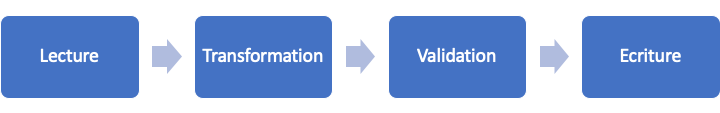
\includegraphics[width=0.7\linewidth]{figures/pipeline_process.png}
    \caption{Structure de fichier présent dans le module de la librairie de l'application. Source : réalisé par Jérôme Chételat}
    \label{fig:pipeline_process}
\end{figure}

Chacun des utilitaires adapte ce pipeline pour traiter des données spécifiques.

\section{Bibliothèque}

La bibliothèque contient les outils de lecture et d'écriture de fichiers pour les formats du chapitre 2.

Elle a comme dépendance principale les crates \textit{stl-io}
qui implémentent les structures pour écrire les fichiers \gls{stl} 
et \textit{las-rs} qui exposent les structures et méthodes liées aux données lidar.

\begin{figure}[htbp!]
    \centering
    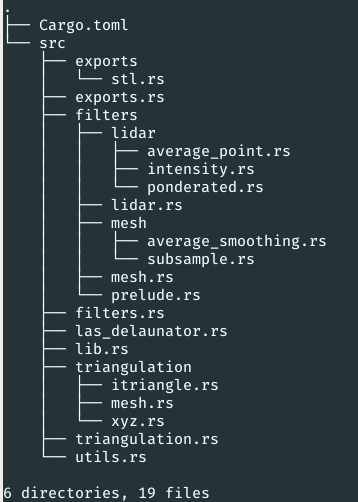
\includegraphics[width=0.5\linewidth]{figures/architecture.png}
    \caption{Structure de fichier présent dans le module de la librairie de l'application. Source : réalisé par Jérôme Chételat}
    \label{fig:library_tree}
\end{figure}

\subsection{Nettoyage}

Les implémentations des filtres sont dérivées du trait \textbf{MeshFilter} ou du trait \textbf{LidarFilter}. Leurs définitions sont les suivantes :
\begin{lstlisting}[language=Rust, style=boxed]
pub trait MeshFilter {
    fn apply(&self, mesh: IndexedMesh, epsilon: f32) -> IndexedMesh;
}

pub trait LidarFilter {
    fn apply(&self, points: Vec<Point>) -> Vec<Point>;
}

\end{lstlisting}

Les traits sont ensuite spécialisés dans le type de filtre voulu.
\subsection{Triangulation}

La librairie contient un module de triangulation.
On y trouve les implémentations des algorithmes de triangulation réalisés lors
du projet de semestre, mais également un algorithme de fusion de triangulation.

\subsubsection{Triangulation de Bowyer-Watson}

L'implémentation a été faite lors du projet de semestre. 
Actuellement l'algorithme a une complexité quadratique ($\mathcal{O}(n^2)$) à cause de la 
recherche d'appartenance d'un point à un triangle qui itère à travers tous les
triangles de la triangulation. Ceci est fait jusqu'à trouver le triangle contenant le point.

Dans ce travail, l'optimisation de cet algorithme n'était pas demandée.
Cependant la complexité pourrait théoriquement être réduite à $\mathcal{O}(n \log(n))$ en
utilisant une structure de données telle qu'un arbre ou un dictionnaire
qui enregistrerait la position des centres des
cercles-circonscrits de chaque triangle créé et parcouru.

\subsubsection{Fusion de triangulation}

Pour la fusion, une structure propre à la librairie était nécessaire en plus des structures de données offertes par la crates \textit{stl-io}.
Elle est définie de la manière suivante:

\begin{lstlisting}[language=Rust, style=boxed]
pub struct Mesh {
    /// Vertices composing the mesh
    pub vertices: Vec<XYZ>,
    /// Indexed triangles of the mesh
    pub faces: Vec<usize>,
    /// Indexed vertices part of the convex hull of the mesh
    pub hull: Option<Vec<usize>>,
    /// The neighbourhood of each indexed point
    pub neighbourhood: Option<Vec<HashSet<usize>>>,
}
\end{lstlisting}

Une particularité de cette structure est que l'on y trouve un champ pour le voisinage du maillage qui est "neighbourhood" et second champ pour l'enveloppe convexe "hull".
Ils sont optionnels pour maintenir une compatibilité avec les crates utilisées dans la librairie.
Une des raisons vient du fait que lors de la lecture d'un fichier \gls{stl}, on ne retrouve pas ces champs. 

Une méthode utile pour s'assurer de la présence d'un voisinage est d'appeler la fonction neighbourhood.
Elle renvoie le voisinage d'un maillage s'il est déjà présent, le cas échéant est de le calculer.

Son implémentation est disponible dans l'annexe 3. 
On parcourt les différents triangles du maillage et pour chaque point présent du triangle, on ajoute ses deux voisins dans un set.

Le set permet de prévenir les duplications de même voisin pour un site. Ce set est ensuite indexé selon le site actuel.

Une fois tout les triangles parcouru, on assigne au maillage le voisinage et l'on renvoie une copie.

Cette dernière peut cependant
être améliorée, car actuellement, une copie du voisinage est renvoyée à
l'appelant. Ce qui à pour effet de créer des données dupliquées dans la mémoire.
Le choix de la copie a été fait, car l'utilisation du voisinage dans un algorithme de fusion nécessite de
muter certaines parties. Une solution pour éviter ces duplications serait de créer
une structure indiquant les parties qui ont muté et de rendre la structure Mesh
immutable. Lors d'un prochain appel de la fonction, cette dernière pourrait
renvoyer un voisinage ayant les changements appliqués à partir de la structure
précédemment décrite.  

Concernant le champ hull, aucune méthode n'est disponible dans la bibliothèque pour en calculer. Il est possible de le calculer au travers de la crate "ncollide" qui expose une version de quickhull, un algorithme de calcule d'enveloppe convexe.

Une fonction intéressante est la recherche d'un candidat final dans un maillage. Voici la signature de la fonction:
\begin{lstlisting}[language=Rust, style=boxed]
fn get_side_candidate(
        mesh: &mut Mesh,
        lr_indexed_point: usize,
        other_lr_point: &XYZ,
    ) -> Option<usize>;
\end{lstlisting}

Elle prend en paramètres un point indexé par un entier non signé dans le maillage passé en argument et une structure de points pour effectuer la recherche puis retourne éventuellement un index pour le site choisi.

Une grosse partie de la fusion est réalisée dans la méthode \textbf{merge} avec comme signature : 
\begin{lstlisting}[language=Rust, style=boxed]
/// Returns a Ok(Mesh) containing the fusion of two meshes togheter.
/// It needs the convex hull of each mesh.
pub fn merge(&mut self, other: &mut Mesh) -> Result<Mesh, &'static str>;
\end{lstlisting}

La méthode renvoie un maillage dans le cas où toute la fusion se serait bien déroulée sinon elle renvoie un message d'erreur.

Une partie intéressante de l'implémentation est la création des arêtes entre la base et un candidat.


Un point intéressant est l'utilisation de pattern matching provenant de langages de programmation fonctionnels pour vérifier les conditions énumérées dans le chapitre 2.3. Si un candidat final est choisi, il est ajouté a une liste d'arêtes \textbf{edges} et à la fin de l'opération, cette liste est utilisée afin de construire les nouveaux triangles entre les deux maillages.

\section{Utilitaires}

Ce module contient les binaires en ligne de commande pour traiter les données du
chapitre 1.
Chaque binaire utilise l'architecture en pipeline, car c'est ce qui s'applique le
mieux pour l'utilisation des outils.

Chaque utilitaire se sert d'une crate pour vérifier et extraire les arguments
donnés à ce dernier. La crate se nomme \textit{clap} et grâce à une macro de la
crate, il est possible de définir simplement les arguments acceptés par 
l'utilitaire.

Voici la liste des commandes disponibles :
\begin{itemize}
	\item las-delaunator : Triangulation par l'algorithme quickhull
	\item las-geometry : Triangulation par l'algorithme de Bowyer-Watson
	\item las-filtering : Nettoyage de points lidar
	\item las-sample : Prendre les $n$ premiers points d'un fichier lidar
	\item las-map-geometry : Triangulation d'un ou plusieurs fichiers
		simultanément
	\item mesh-merge : Fusion de maillage
	\item mesh-smoothing : Nettoyage de maillage
	\item mesh-subsample : Prendre qu'une partie des triangles du maillage
	\item to-txt : Transforme un fichier lidar en simples points ASCII dans le
		format $x\ y\ z$
\end{itemize}

\subsection{mesh-smoothing}

Le binaire ici produit permet de nettoyer le bruit qui est généré par les points
lidars après une triangulation. Il agit sur les triangles d'un maillage.

La commande prend en argument un fichier d'entrée et un fichier de sortie. Il
prend également en option un paramètre $\epsilon$ qui sert de critère pour
appliquer la moyenne d'un point par rapport à ses voisins.

Pour réaliser le nettoyage, on itère à travers la liste des sommets du maillage.
Pour chaque sommet, on vérifie si la différence entre la hauteur moyenne des voisins
et le sommet actuel est inférieure au $\epsilon$.
Si la condition est vraie, dans ce cas on assigne la hauteur moyenne des voisins
au sommet actuel. Le cas échéant, le sommet est simplement ignoré.

L'itération se fait sur une copie des sommets du maillage pour éviter d'avoir
des incohérences de hauteurs avec les points voisins dans le cas où un sommet
voisin d'un autre est modifié avant ce dernier.

\subsection{mesh-subsample}

La commande permet de décimer un maillage. Elle
prend en argument un fichier STL d'entrée et un fichier STL de sortie.
Elle prend encore en paramètres optionnels un type de filtre à appliquer.

Le paramètre du choix de la méthode de décimation est un nombre.

\begin{enumerate}
	\item Décimation par rapport à la distance
	\item Décimation aléatoire
\end{enumerate}

Par défaut, si aucune méthode n'est choisie, on applique la décimation selon la
distance.

On crée un itérateur sur les sommets présents dans le fichier STL. Ensuite on
calcule la distance euclidienne par rapport au voisin de chaque sommet.
Si elle se trouve être inférieure à la valeur de $\epsilon$, on supprime le
sommet. Après avoir déterminé les sommets qui sont à garder, on applique à
nouveau une triangulation quickhull de la crate \textit{delaunator-rs}. Enfin on
retourne le nouveau maillage contenant moins de sommets. 
Une autre manière de
choisir quels points seront supprimés est de le faire aléatoirement.

\subsection{mesh-merge}

Cette commande permet à un utilisateur de créer une triangulation à
partir de la fusion de deux triangulations existantes. Cet outil est
particulièrement utile lors de lorsque l'on a déjà une partie des points lidar
sous forme de maillage.
\section{Stack Web}

Cette section présente la partie concernant le web. On y détaille l'implémentation
de deux modules: le client et le serveur.
Ces derniers forment le \textit{stack web}.

\subsection{Serveur}

Le serveur consiste en un binaire Rust utilisant le framework actix-web.
Le choix de l'utilisation de ce framework a été fait pour déléguer la gestion des
requêtes reçues de bas niveau ainsi que l'utilisation simple de fonctions
asynchrones pour gérer ces dernières.
Il a aussi été choisi, car il est le seul pour l'instant à utiliser que des fonctionnalités stables du langage de programmation.

Le serveur est une \gls{api} \gls{rest} comprenant une route pour chaque fichier
d'un dossier.
Elle expose au web, les fichiers appartenant au dossier nommé \textit{regions}.
Ce dernier pouvant être donné en argument au serveur, à son lancement.

Concernant les mécanismes de \gls{cors}, on utilise une crate de actix
s'appelant \textit{actix\_cors}.
Il s'agit d'un middleware actix s'ajoutant sur une ou plusieurs routes pour
activer les mécanismes \gls{cors}.

La lecture et le découpage en paquet d'un fichier sont réalisés par un autre
module de actix.
% et parce qu'il se trouve être le seul framework web pour Rust
% n'utilisant pas une version instable du compilateur de Rust. Il a aussi été
% choisi, car il permet une mise en oeuvre simple de fonctions asynchrones traitant
% les requêtes.
% Le serveur est une application binaire qui utilise le framework actix-web.
% Ce framework utilise les nouvelles fonctionnalités du langage telles que les async/await sur des routes.
% Il s'agit donc d'une \gls{api} de \gls{rest} exposant une seule route pour récupérer les fichiers de manière statique. Un futur projet pourrait construire un service de triangulation ou encore un service de filtrage.

\subsection{Client}

Le client web a été écrit en Rust et compilé en \gls{wasm}.
Il permet une visualisation de maillage au travers d'un navigateur web grâce à
la bibliothèque graphique WebGL.
% Les rendu des maillages se fait par l'api WebGL. WebPack, un packager d'application web, a été utilisé pour liés le HTML, le JavaScript et les modules \gls{wasm}. 

Cette partie utilise grandement une crate appelée "web-sys" qui expose des bindings pour le JavaScript.
On utilise également la crate "nalgebra" qui propose des fonctions pour manipuler des matrices 4x4 utilisées dans WebGL.

Lorsqu'on écrit du code Rust ciblant les plateformes web, plusieurs contraintes
doivent être respectées. La première est que \gls{wasm} étant un format sur 32
bits, la mémoire adressable par le programme n'est que de quatre gigaoctets. Une
seconde contrainte est que les threads n'existent pas pour une application web
et sont remplacés par les WebWorkers
\footnote{Technologie des navigateurs web permettant l'exécution de
code dans un processus en arrière-plan de manière indépendante}.
% Une contrainte survient en écrivant du code pour le web avec Rust est que la plupart des fonctionnalités pour améliorer le fonctionnement des modules sont à ce jour encore expérimental et de ce fait, pas suffisamment stable pour créer une application complète.

Lors du chargement de la page web, la première étape est de récupérer le fichier
qui doit être affiché.
Ceci est fait à partir de l'\gls{api} \textit{fetch} des
navigateurs. On forge un objet requête en donnant le lien de téléchargement du
fichier. Une fois téléchargé, on transforme la réponse en \textit{blob}.
Ce dernier est ensuite casté en tableau Rust à travers la crate \textit{JsCast}.
La lecture du fichier \gls{stl} en binaire est déléguée à la crate \textit{stl-io}.

On récupère les vertex du maillage ainsi que les indices des sommets qui forment les
triangles. On récupère aussi les normales des triangles. Ils nous permettront de
faire le calcul des ombrages.

On crée ensuite un vertex buffer object pour chaque objet récupéré du
maillage, puis l'on transfère les données dans les buffers respectifs.
Cette dernière opération en Rust est dans un bloc \textit{unsafe}, car on déréférence des
pointeurs dans la mémoire du navigateur.
Enfin on crée les matrices de projection, de vue et de transformation 
puis on les transfère également dans des zones mémoires graphiques.
Enfin on ordonne de faire un rendu à l'écran.
